%
% Documento: Abordagem e modelagem do Problema
%

\chapter{Abordagem e Modelagem do Problema}
\label{chap:abordagememdelo}
Existem diversas maneiras de se implementar um sistema como este, tanto do ponto de vista do sistema distribuído e sua rede de comunicação, quanto do ponto de vista de controle e realimentação das malhas. Neste capítulo faz-se um detalhamento da abordagem do problema e do funcionamento do sistema como um todo e a modelagem escolhida para abordar o problema. Será utilizado uma abordagem já mencionada anteriormente, que é o controle em cascata, utilizado para modularizar o problema e assim, tornar mais simples a implementação e o entendimento do mesmo. 

Serão três malhas de controle: A primeira e mais interna será responsável pelo controle da velocidade angular de cada roda, para se chegar à posição (\emph{x,y}) desejada. Esta malha estará presente em cada um dos robôs da frota que estarão à circular o alvo. A segunda, malha intermediária, será responsável para que cada robô chegue à um determinado ponto (\emph{x,y}) no espaço, portanto, será responsável por corrigir o posicionamento do robô. Esta malha também estará presente em cada robô que circundar o alvo. A terceira malha, e portanto, a mais externa é responsável pela coordenação da frota, fornecendo a cada robô as informações necessárias para que o mesmo saiba o ponto (\emph{x,y}), onde deve ficar para consolidar e manter a formação.

Faz-se então neste capítulo, primeiramente, a modelagem do problema. Para que então, possa-se modelar as malhas de controle e estabelecer a modelagem da rede de comunicação da frota, que não será modelada nesta primeira etapa do trabalho. Portanto, não serão apresentados detalhes sobre ela. Para estabelecer o modelo matemático do problema, será considerado o modelo de robô mostrado na \autoref{fig:robo}.

\begin{figure}[!htb]
	\centering
	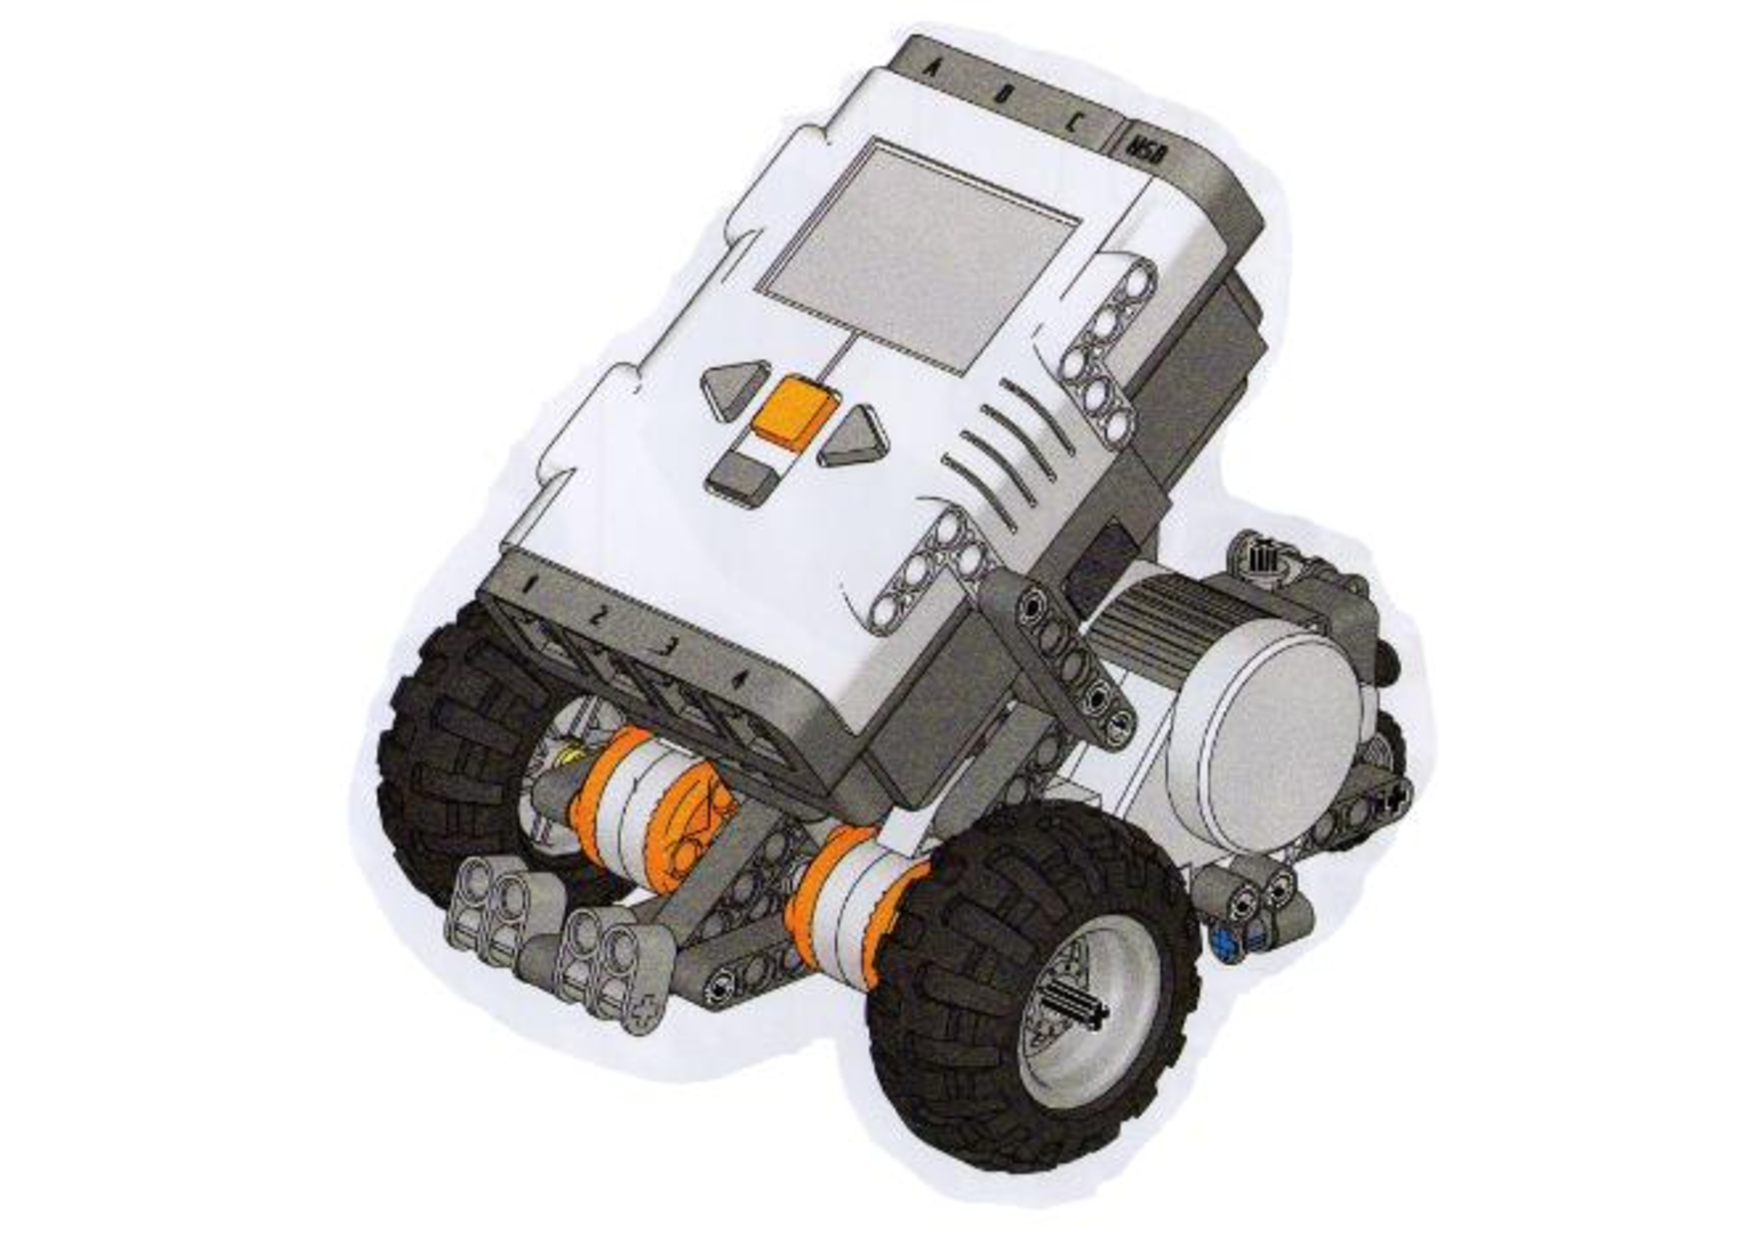
\includegraphics[width=10cm]{./04-figuras/robo}
	\caption{Modelo do Robô}
	\label{fig:robo}
\end{figure}
 

\section{Modelo Matemático}
\label{sec:modMatematico}
Este trabalho tem como intuito modelar uma malha de controle que guie uma frota de robôs a circundar, a uma distancia \emph{R}, um alvo localizado em uma determinada posição (\emph{x,y}) do plano. Esse controle deve, também, ser responsável pela formação da tropa de robôs que, com a falha de um ou mais robôs, deve se reestruturar para continuar cobrindo com eficiência a fronteira. Ou seja, caso um ou mais robôs saiam da rede, a frota ira se reajustar para que cada robô tenha a mesma distância entre si e assim, não fique uma grande parte da fronteira sem cobertura, como demostrado na \autoref{fig:sistema}. Que representa uma frota de quatro robôs andando ao redor do alvo, quando então, um dos robôs falha. E o sistema se reajusta para adaptar-se à rede de apenas três robôs.

\begin{figure}[!htb]
	\centering
	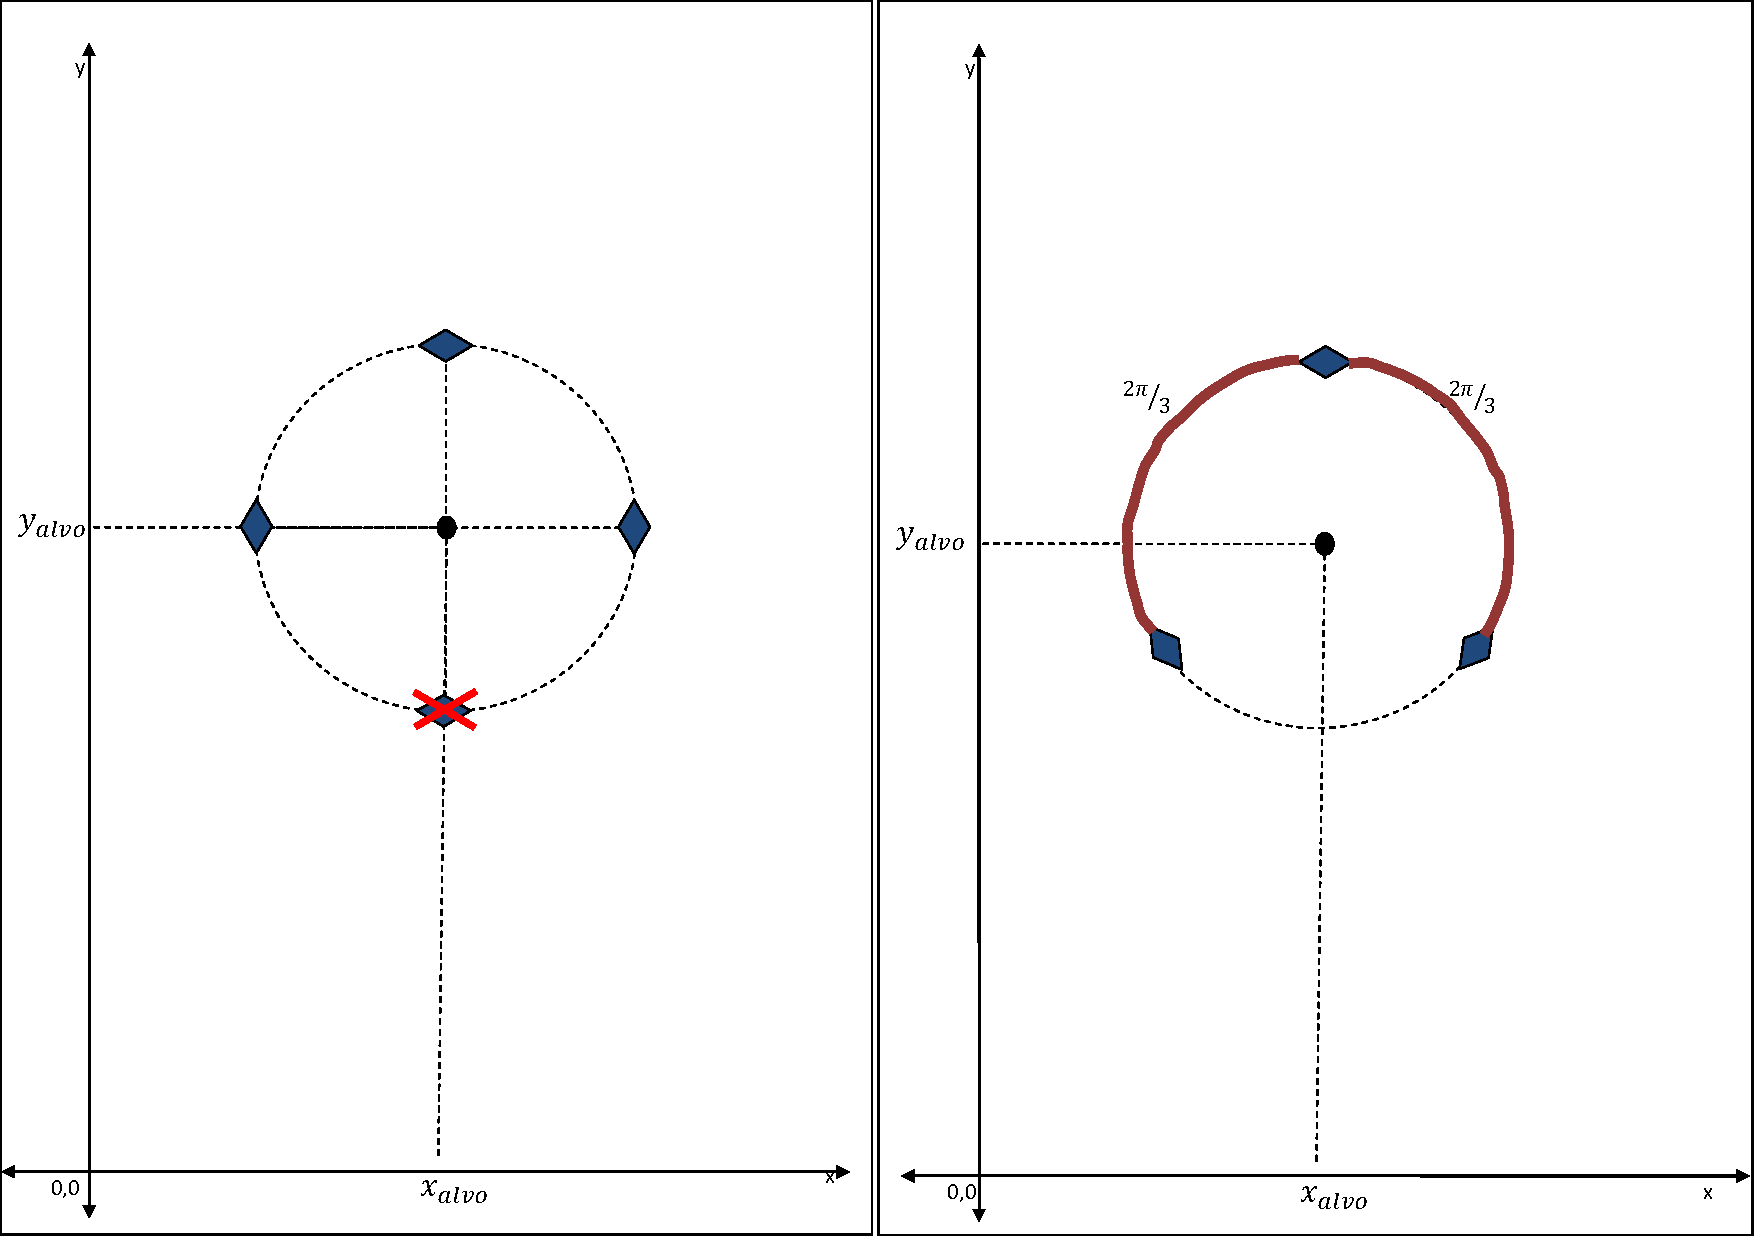
\includegraphics[width=1.0\textwidth]{./04-figuras/sistema}
	\caption{Modelagem do Sistema}
	\label{fig:sistema}
\end{figure}

Para introduzir a dinâmica dos robôs móveis utilizados, inicialmente o robô será considerado como um uniciclo, um elemento pontual. A dinâmica de um robô móvel não-holonômico do tipo uniciclo, desconsiderando a dinâmica, pode ser descrita pelas equações abaixo:

\begin{equation}
\dot{x} = v\cos(\theta) 
\label{eq:posiçãox}
\end{equation}
\begin{equation}
\dot{y} = v\sin(\theta)
\label{eq:posiçãoy}
\end{equation}
\begin{equation}
\dot{\theta} = \omega
\label{eq:posiçãotheta}
\end{equation}

sendo:
\begin{itemize}
	\item ($x$,$y$) as coordenadas da posição do robô no plano cartesiano;
	\item $\theta$ o sentido do robô no plano cartesiano;
	\item $v$ e $\omega$ indicam a velocidade linear e angular do robô, respectivamente.	
\end{itemize}

Derivadas dessas equações, surgem as equações \ref*{eq:posiçãoxreal},\ref*{eq:posiçãoyreal} e \ref*{eq:posiçãothetareal} modeladas baseadas no robô real, que não é um elemento pontual no espaço e sim, um modelo não holonômico. Elas serão utilizadas a princípio para visualizar a trajetória do robô no ambiente \emph{MATLAB\textregistered}.

\begin{equation}
x_{k+1} = x_{k} + \dfrac{D_{r} + D_{l}}{2}\cos(\theta_{k}) 
\label{eq:posiçãoxreal}
\end{equation}
\begin{equation}
y_{k+1} = y_{k} + \dfrac{D_{r} + D_{l}}{2}\sin(\theta_{k}) 
\label{eq:posiçãoyreal}
\end{equation}
\begin{equation}
\theta_{k+1} = \theta_{k} + \dfrac{D_{r} - D_{l}}{L}
\label{eq:posiçãothetareal}
\end{equation}

sendo:
\begin{itemize}
	\item $x_{k+1}$ e $x_{k}$ a coordenada $x$ do robô no instante $k$ e no instante $k+1$;
	\item $y_{k+1}$ e $y_{k}$ a coordenada $y$ do robô no instante $k$ e no instante $k+1$;
	\item $\theta_{k+1}$ e $\theta_{k}$ o sentido do robô no instante $k$ e no instante $k+1$;	
	\item $D_{r}$ e $D_{l}$ a distância que a roda direita e esquerda percorreram no instante de tempo entre $k$ e $k+1$, respectivamente;
	\item $L$ o tamanho do eixo do robô;
\end{itemize}

Considerando que à medida que o sistema se estabiliza, o robô tende entra em movimento circular uniforme ao redor do alvo. Ou seja, a velocidade linear ($v$) tende a se igualar a velocidade angular ($\omega$) vezes o raio ($R$) de distância do alvo.

\begin{figure}[!htb]
	\centering
	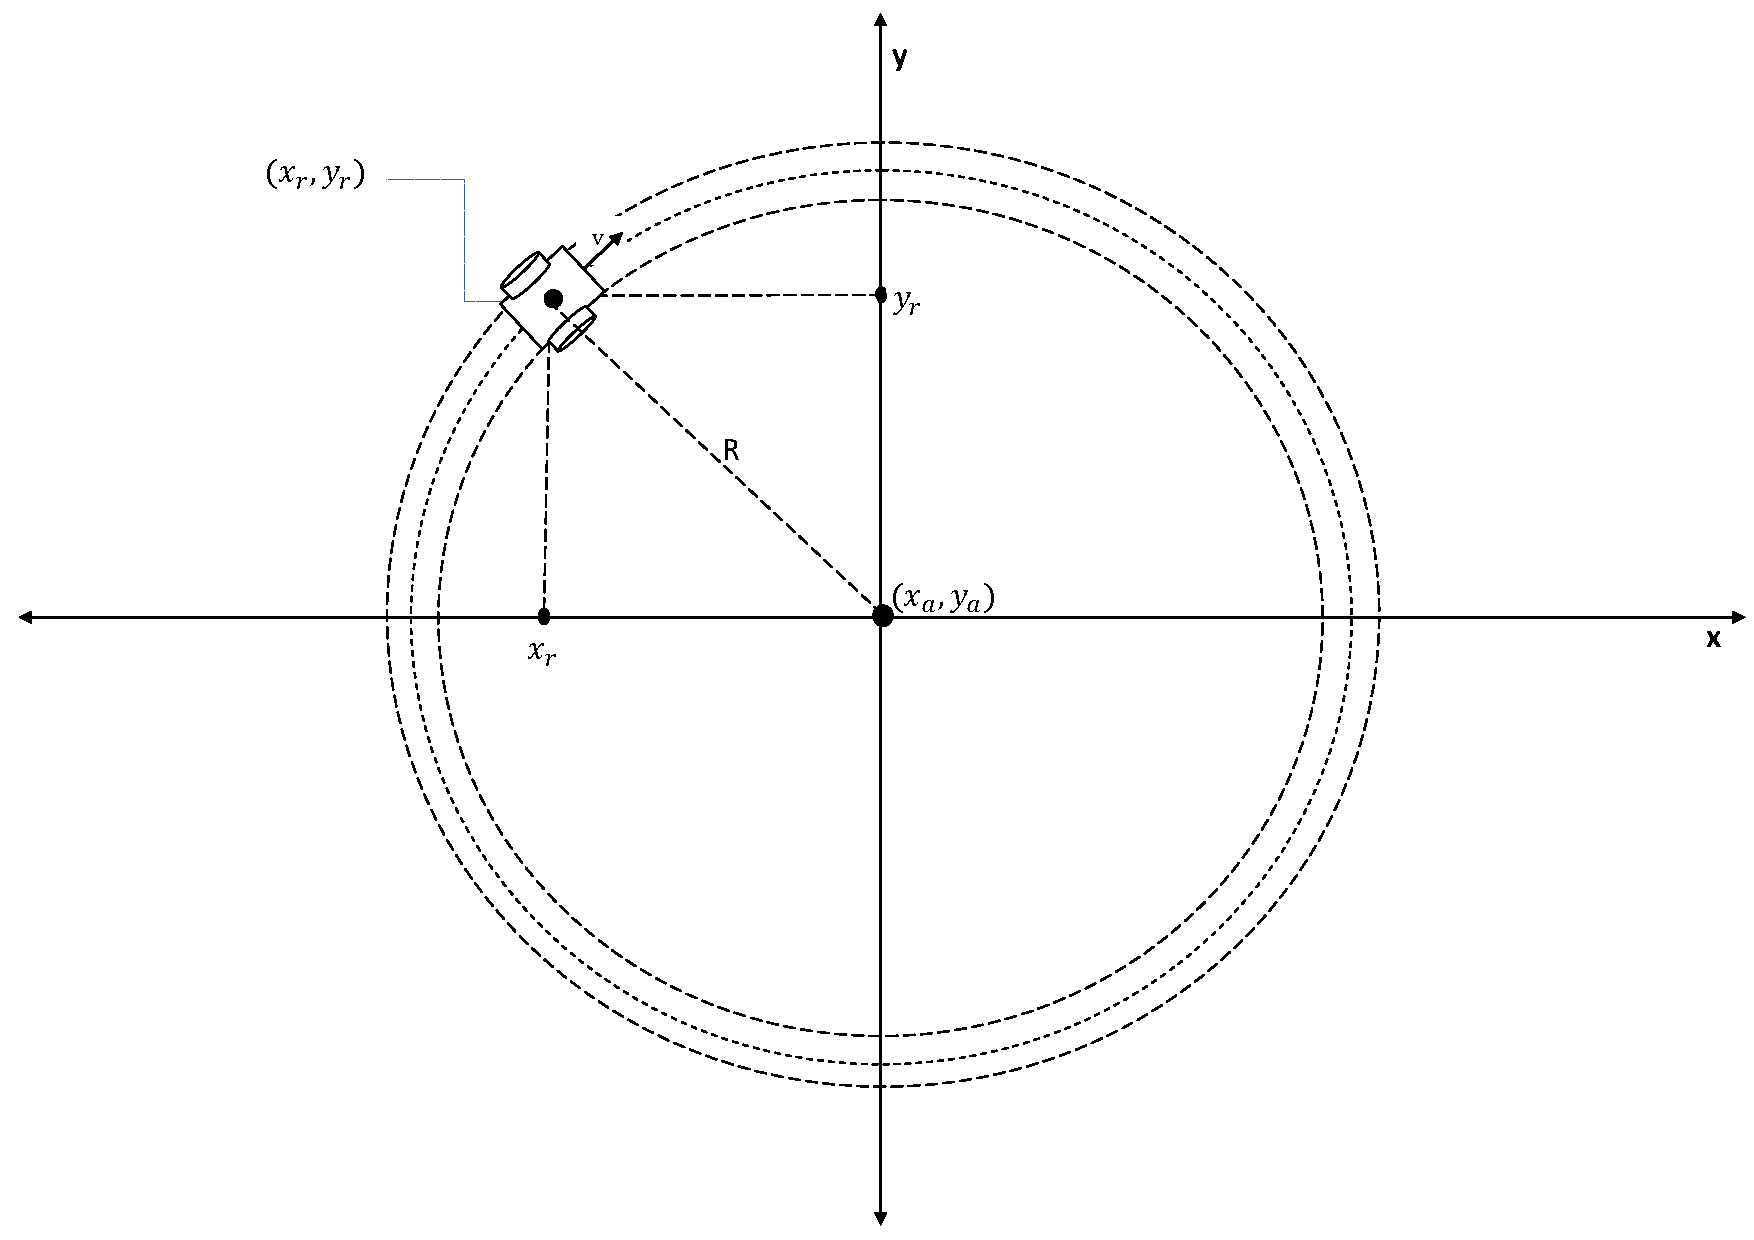
\includegraphics[width=1.0\textwidth]{./04-figuras/sistEstavel2}
	\caption{Representação do sistema estável}
	\label{fig:sistEst}
\end{figure}

\section{Malha de Controle 2: Posicionamento}
\label{sec:malha2 } 
O trabalho tem como objetivo, dado a posição \emph{x,y} do alvo ($x_{a},y_{a}$), fazer com que a frota de robôs se desloque para a região no espaço do alvo e o circule com uma distância \emph{R}, à uma dada velocidade angular ($\omega_{d}$) desejada. Para que a malha de controle 3, que consiste no controle de formação da tropa funcione, primeiramente é necessário, implementar o controle de posicionamento de cada robô da frota. Ou seja, a malha de controle de formação irá passar para cada robô os parâmetros necessários para o ajuste da estrutura, tais como, velocidade e posicionamento.%definir aqui DEPOIS como será esse controle, se será uma simulação de uma rede distribuida, se será uma rede distribuida de fato, ou se será apenas uma rede centralizada

Como pode ser visto na \autoref{fig:esq2}, o problema a ser solucionado pela segunda malha de controle, consiste em, dado um sistema de coordenadas cartesianas, onde têm-se um alvo de posição (\emph{$x_{a},y_{a}$}) e um robô móvel de posição (\emph{$x_{r},y_{r}$}), cujo sentido (\emph{$\theta$}) é indicado pela sua variação dado o eixo \emph{x} do sistema, onde pretende-se fazer com que o robô chegue ao ponto desejado (\emph{$x_{d},y_{d}$}, recebido da malha de controle 3), que se distância do alvo à uma distância \emph{R}, e então, fazê-lo circular ao redor do alvo. Ou seja, consiste em fazer com que o robô vá até o alvo e o circule à uma distância \emph{R}.
	   
\begin{figure}[!htb]
	\centering
	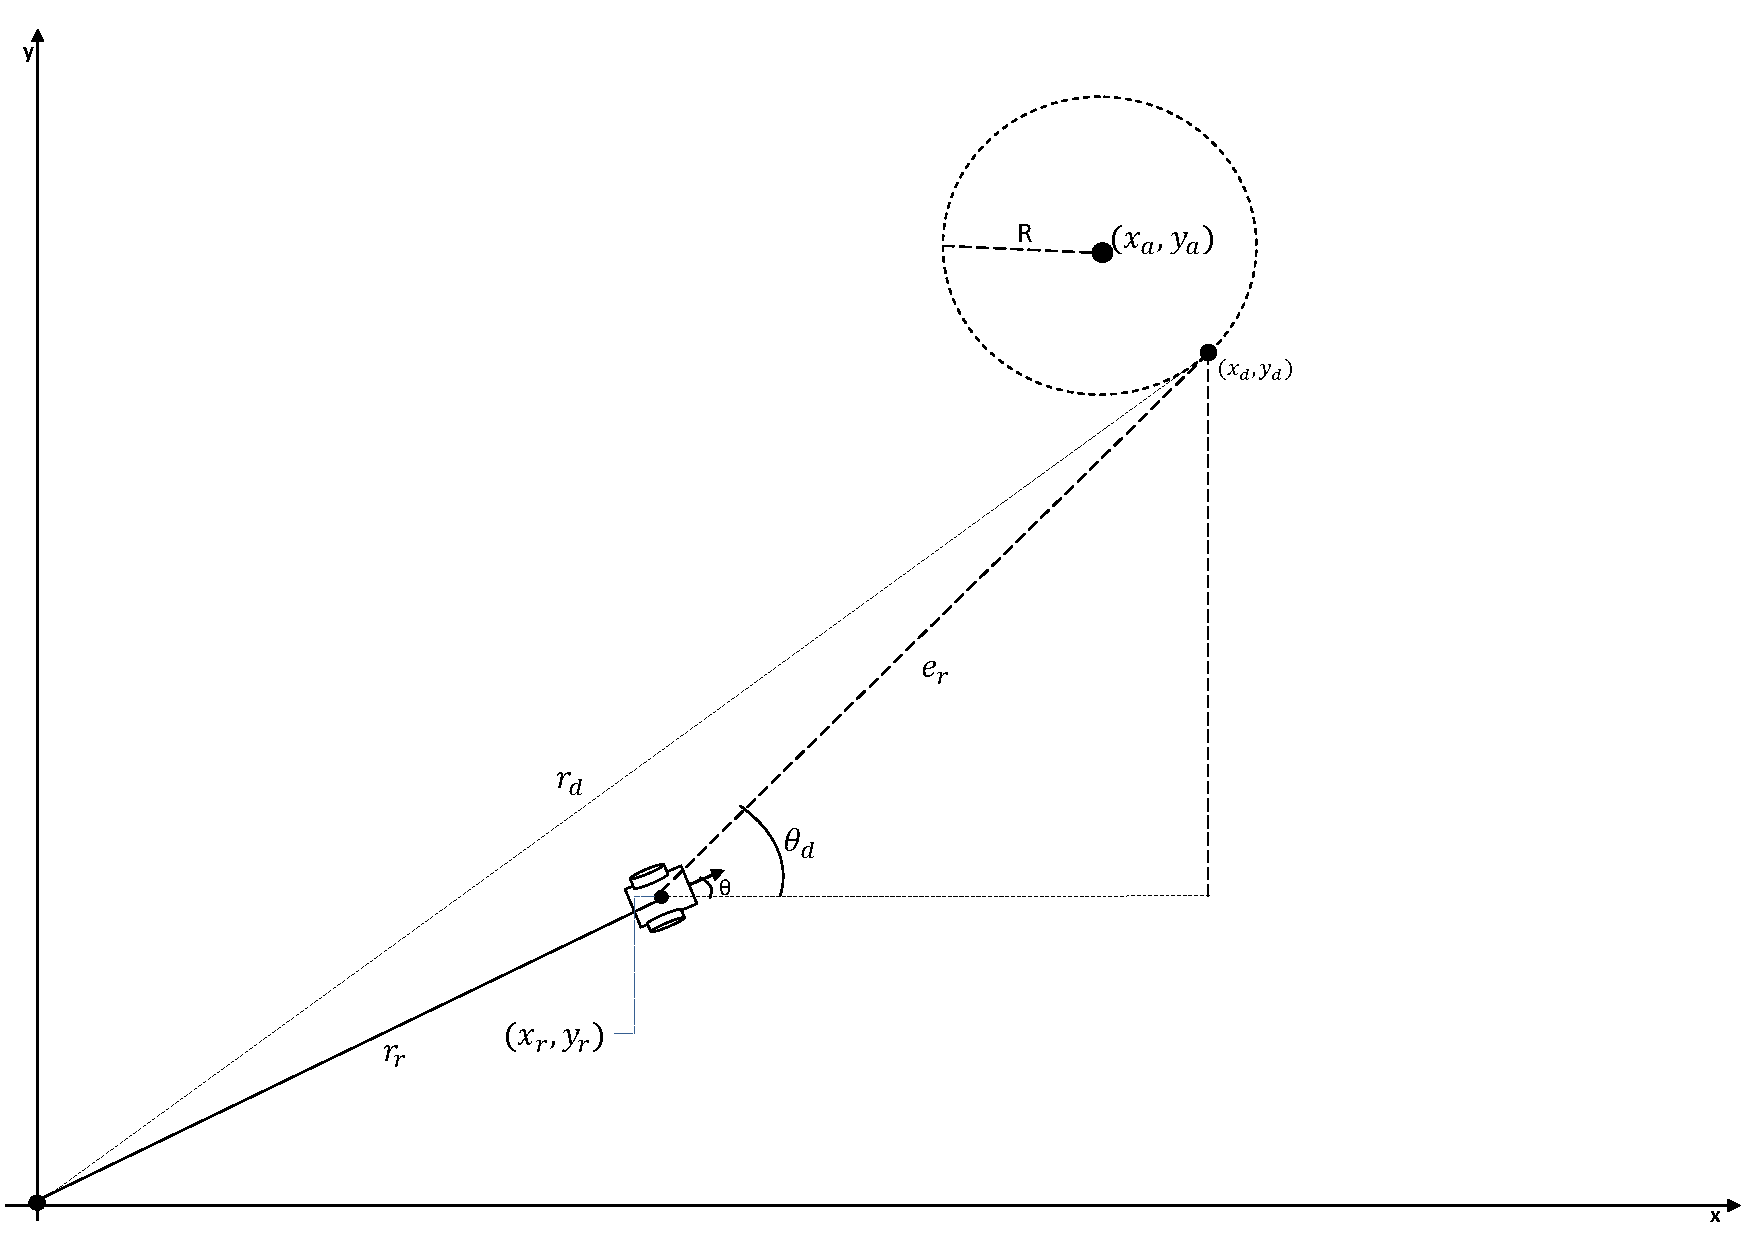
\includegraphics[width=1.0\textwidth]{./04-figuras/esqSistema}
	\caption{Esquema do Sistema do Ponto de Vista de Apenas Um Agente}
	\label{fig:esq2}
\end{figure}

Para tal, a malha 2 funciona da da seguinte maneira: Recebe da malha 3 os parâmetros necessários para o cálculo da posição desejada do robô (\emph{$x_{d},y_{d}$}), a partir daí é achado o erro de posição do robô (\emph{$e_{x},e_{y}$}), fazendo-se a diferença entre a posição desejada e a posição real do robô (\emph{$x_{r},y_{r}$}), que é obtida através dos \emph{encoders} do LEGO\textregistered, que se mostrou suficientemente precisos.

\begin{equation}
e_{r} = r_{d} - r_{r}
\label{eq:errr}
\end{equation}
\begin{equation}
e_{x} = x_{d} - x_{r}
\label{eq:errx}
\end{equation}
\begin{equation}
e_{y} = y_{d} - y_{r}
\label{eq:erry}
\end{equation}

Através do erro de posicionamento do robô, encontra-se o sentido desejado (\emph{$\theta_{d}$}), como mostrado na \autoref{eq:thetad}. Então, o erro de sentido do robô é obtido, através da \autoref{eq:errtheta} abaixo. 

\begin{equation}
\theta_{d} = \arctan(\dfrac{e_{y}}{e_{x}})
\label{eq:thetad}
\end{equation}
\begin{equation}
e_{\theta} = \theta_{d} - \theta_{r}
\label{eq:errtheta}
\end{equation}

O erro de sentido (\emph{$e_{\theta}$}) é passado para o controlador que retorna a velocidade angular da ação de controle, que será passada para a malha mais interna. Posteriormente, será feita uma comparação entre os controladores \emph{PI} e \emph{PID} e será definido o controlador a ser utilizado nesta malha.

\begin{figure}[!htb]
	\centering
	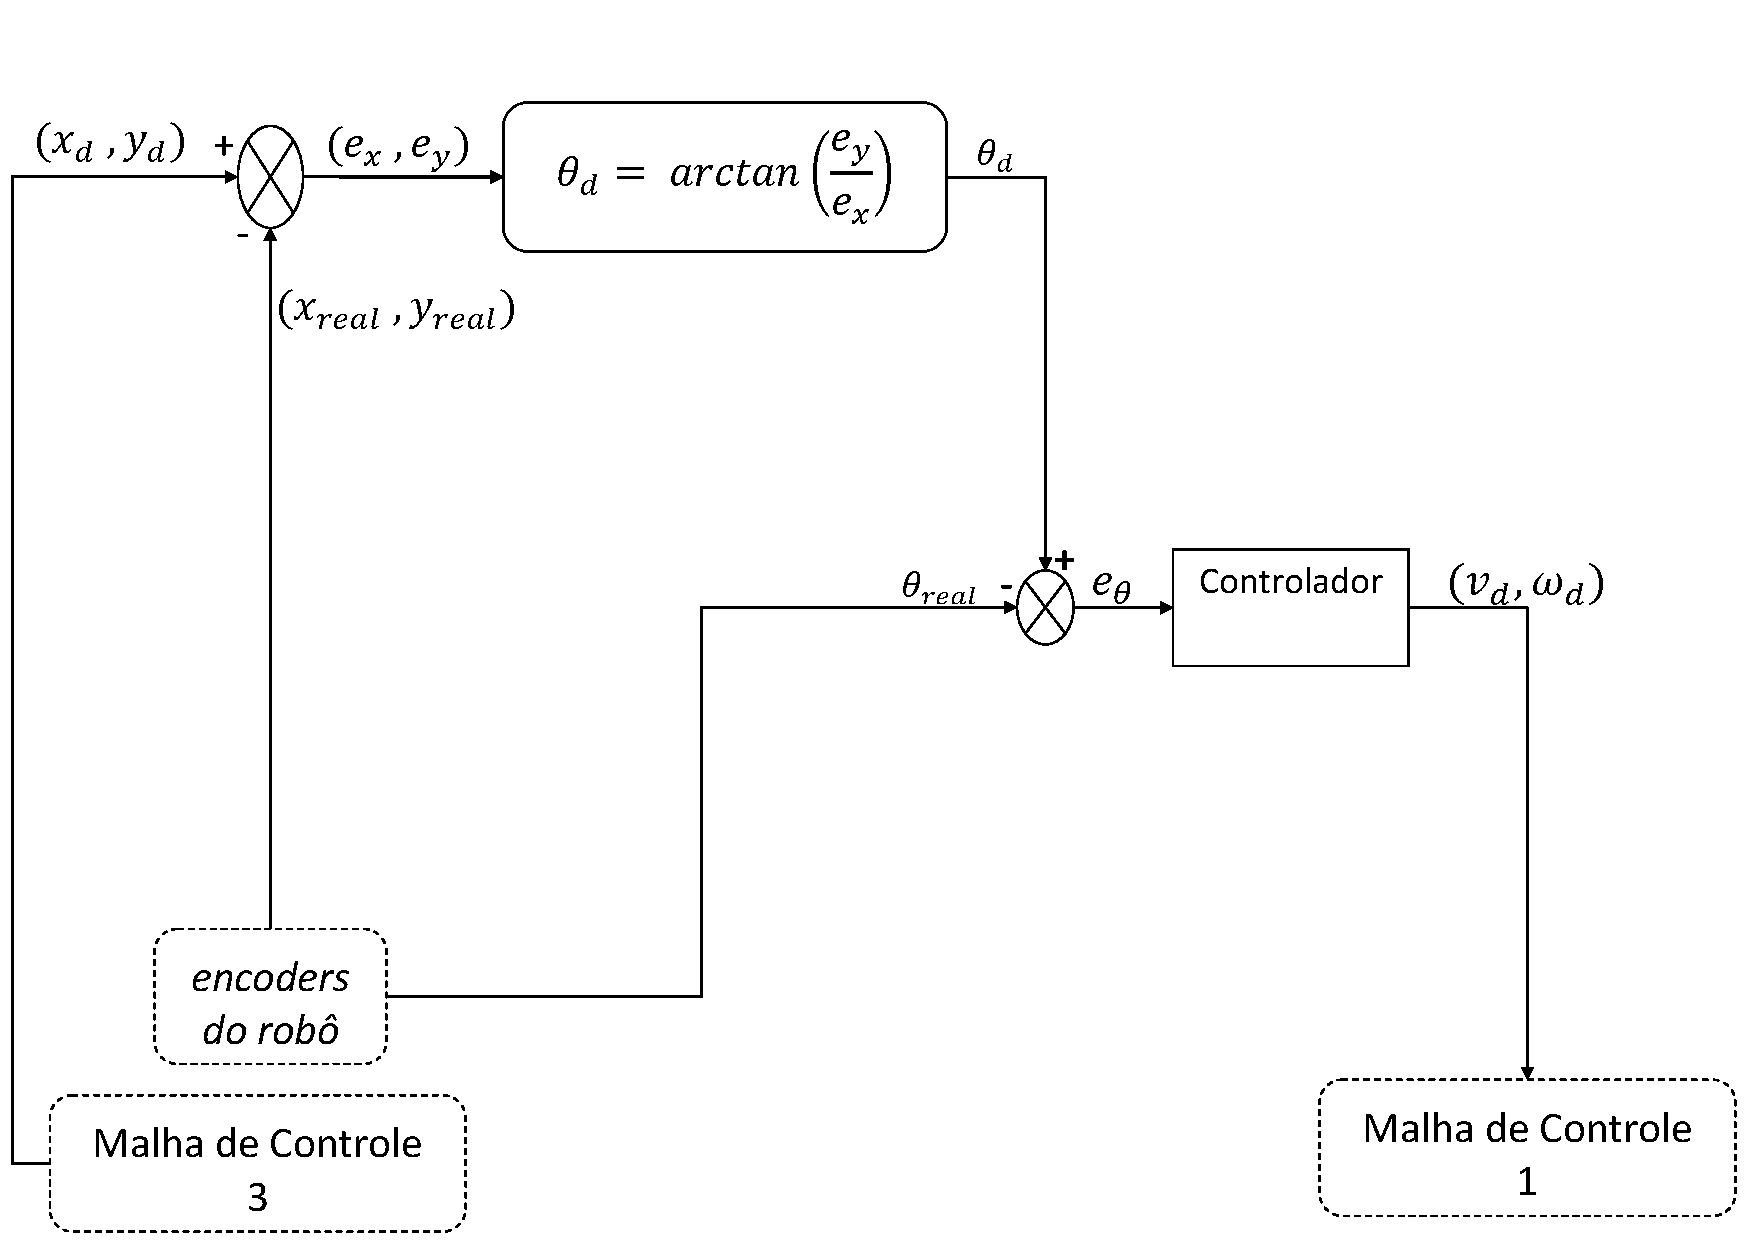
\includegraphics[width=1.0\textwidth]{./04-figuras/malha2}
	\caption{Segunda malha de Controle do Sistema - Controle de Posicionamento}
	\label{fig:malha2}
\end{figure}

 
\section{Malha de Controle 1: Velocidade Angular das Rodas}
\label{sec:malha1 } 
Como já dito anteriormente neste trabalho, este sistema de controle consiste em um controle de três malhas, e agora será abordado sobre a primeira malha. Ela controla os motores para atingir a velocidade angular desejada ($ \omega _{d} $). Ou seja, deseja-se circular o alvo em um período de \emph{T} segundos, a malha de controle de velocidade vai receber a velocidade angular desejada ($ \omega _{d} $), que é uma derivação do período de circulação desejado, como mostrado na equação abaixo:
\begin{equation}
\omega = \dfrac{2\pi}{T}
\label{eq:velocangular}
\end{equation}
É importante ressaltar que como o robô não é um elemento pontual\footnote{Veja a \autoref{fig:sistEst} para visualizá-lo como um elemento não pontual, que depende da variação de velocidade de cada roda para definir a velocidade e o sentido do robô.}, como considerado na \autoref{sec:modMatematico} ao descrever as equações do modelo, temos que descrever a velocidade angular (\emph{$\omega$}) e linear (\emph{$v$}) do robô em função de cada roda, para sabermos a potência a ser aplicada em cada uma delas para que o robô obtenha a velocidade e o sentido desejados.

A partir daí o módulo calcula velocidade angular desejada de cada roda, como demonstrado nas equações abaixo:
\begin{equation}
\omega_{dr} = \dfrac{2v + \omega_{d}L}{2r_{p}}	
\label{eq:velocangulardireita}
\end{equation} 
\begin{equation}
\omega_{dl} = \dfrac{2v - \omega_{d}L}{2r_{p}}	
\label{eq:velocangularesquerda}
\end{equation} 

onde:
\begin{itemize}
	\item $v$ é a velocidade linear (m/s) desejada do robô;
	\item $\omega_{dr}$ é a velocidade angular desejada da roda direita;
	\item $\omega_{dl}$ é a velocidade angular desejada da roda esquerda;
	\item $r_{p}$ o raio do pneu (m);
	\item $L$ o tamanho do eixo do robô (m).	
\end{itemize}

Com a velocidade angular de cada roda, dada pelos \emph{encoders} do robô, é calculado o erro das velocidades, como mostrado nas equações abaixo, e o controlador \emph{PI}, os recebe como entrada, retornando as ações de controle que serão passadas como potência para cada uma das rodas.
\begin{equation}
e_{wr} = \omega_{dr} - \omega_{rr}
\label{eq:errVelAngDireita}
\end{equation} 
\begin{equation}
e_{wl} = \omega_{dl} - \omega_{rl}
\label{eq:errVelAngEsquerda}
\end{equation} 

onde:
\begin{itemize}
	\item $e_{wr}$ é o erro da velocidade angular da roda direita;
	\item $e_{wl}$ é o erro da velocidade angular da roda esquerda;
	\item $\omega_{rr}$ é a velocidade angular real da roda direita;
	\item $\omega_{rl}$ é a velocidade angular real da roda esquerda.	
\end{itemize}	

\begin{figure}[!htb]
	\centering
	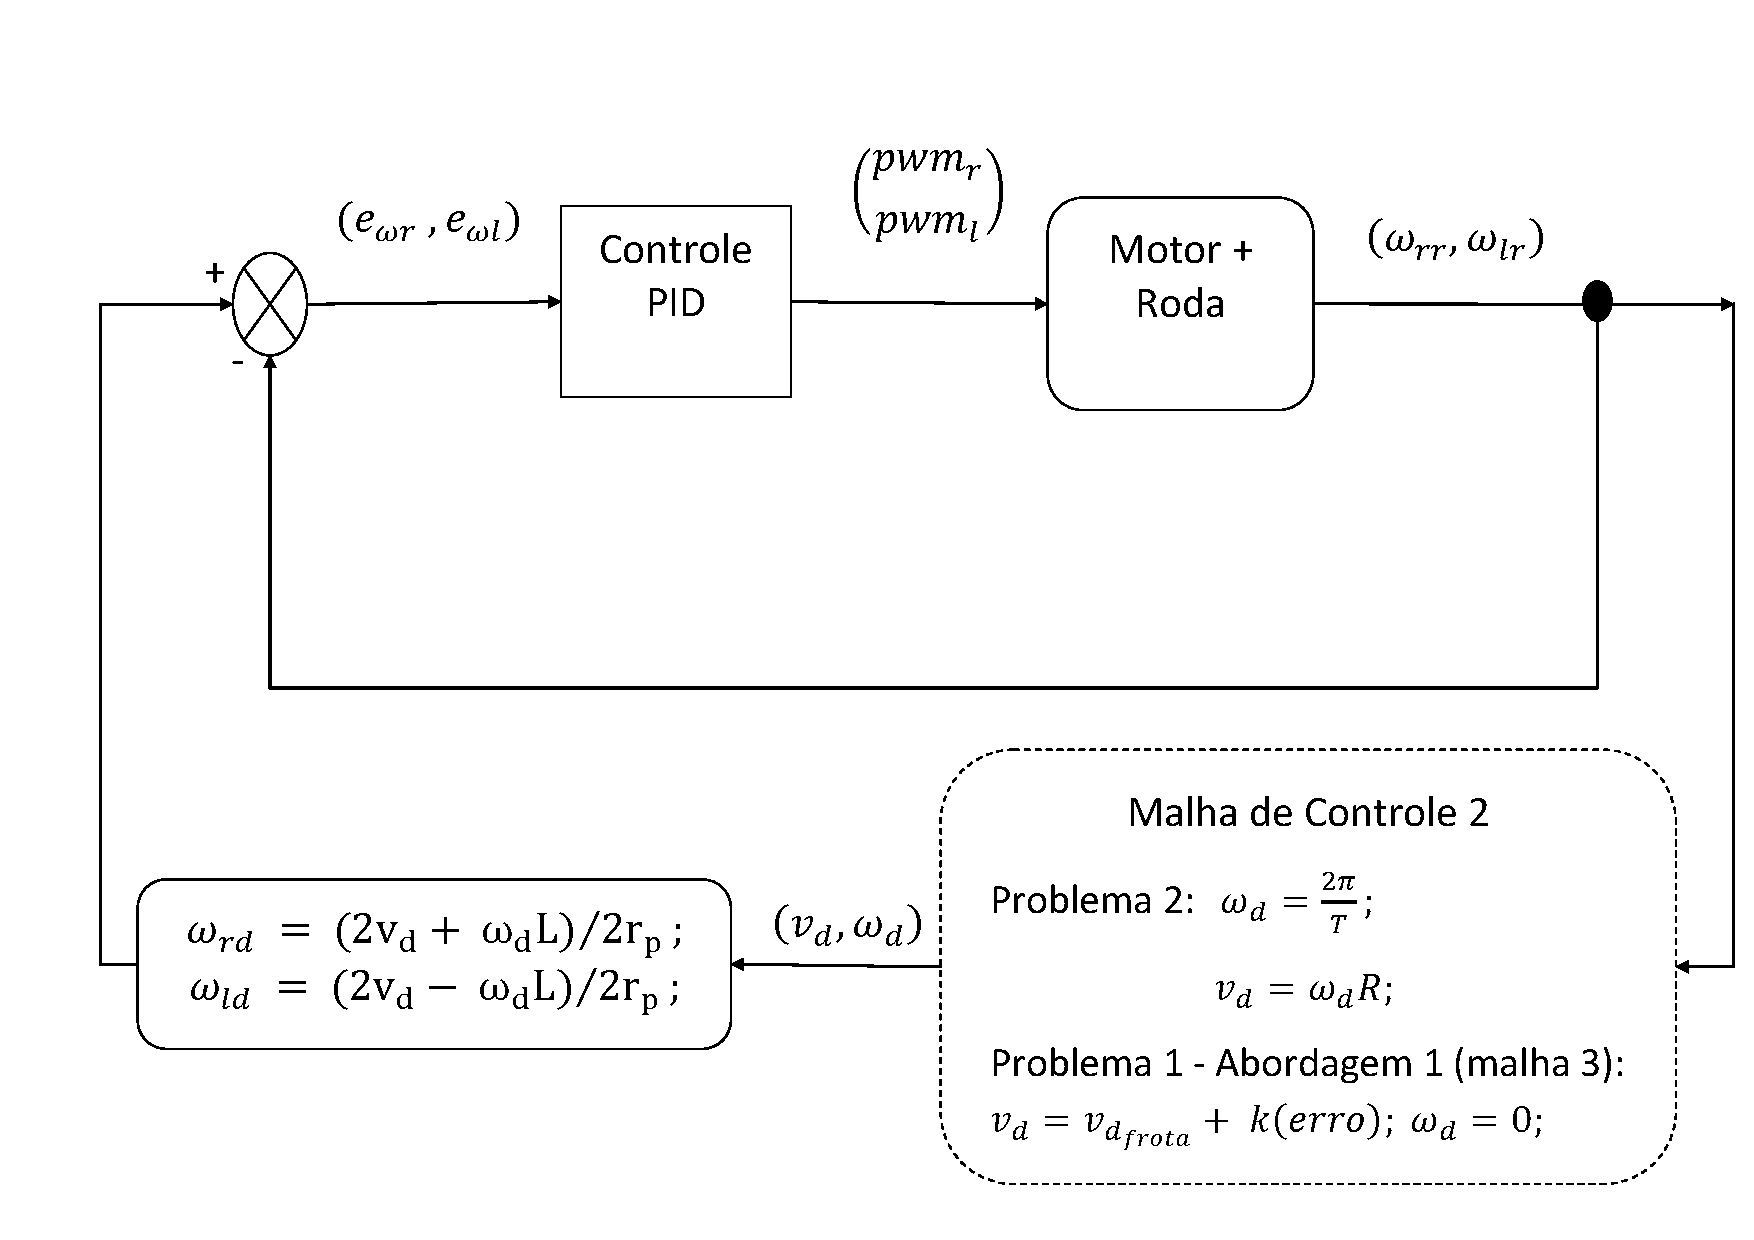
\includegraphics[width=1.0\textwidth]{./04-figuras/malha1}
	\caption{Primeira malha de Controle do Sistema - Controle da velocidade angular}
	\label{fig:malha1}
\end{figure}

